\begin{center}
    \textbf{Geração 20}
\end{center}

\begin{figure}[h]
    \centering
    \label{fig:geracao01}
    
    \begin{tabular}{rl}
        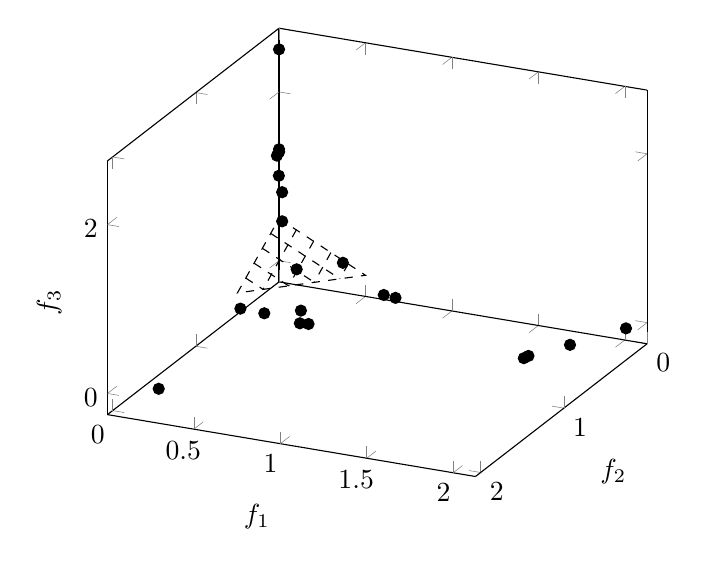
\begin{tikzpicture}[scale=1.0]
        	\begin{axis}[xlabel=$f_2$, ylabel=$f_1$, zlabel=$f_3$, view/h=115]
        		
    			\addplot3[style={dashed}]coordinates {
    			    (0., 0., 0.5) (0., 0.5, 0.) (0.5, 0., 0.) (0., 0., 0.5)
    			};
    			
    			\addplot3[style={dashed}]coordinates {(0., 0.1, 0.4) (0.4, 0.1, 0.)};
    			\addplot3[style={dashed}]coordinates {(0., 0.2, 0.3) (0.3, 0.2, 0.)};
    			\addplot3[style={dashed}]coordinates {(0., 0.3, 0.2) (0.2, 0.3, 0.)};
    			\addplot3[style={dashed}]coordinates {(0., 0.4, 0.1) (0.1, 0.4, 0.)};
    			
    			\addplot3[style={dashed}]coordinates {(0.4, 0., 0.1) (0.4, 0.1, 0.)};
    			\addplot3[style={dashed}]coordinates {(0.3, 0., 0.2) (0.3, 0.2, 0.)};
    			\addplot3[style={dashed}]coordinates {(0.2, 0., 0.3) (0.2, 0.3, 0.)};
    			\addplot3[style={dashed}]coordinates {(0.1, 0., 0.4) (0.1, 0.4, 0.)};
    			
    			\addplot3[only marks] coordinates {
            		(0.196283, 0.196542, 0.115822) (0.269935, 0.735743, 0.053505) (0.031118, 0.033150, 0.502100) (0.752572, 0.276971, 0.046618) (0.003142, 0.002071, 1.292353) (0.280071, 0.808486, 0.052340) (0.589592, 0.410344, 0.000000) (0.806199, 0.164489, 0.103897) (0.000000, 0.000000, 1.320581) (0.008603, 0.003156, 1.014277) (0.753674, 0.483285, 0.000000) (0.253436, 2.128926, 0.125329) (2.062402, 0.296612, 0.157661) (0.000000, 0.000000, 2.503756) (0.732450, 1.768525, 0.013297) (0.745924, 0.529591, 0.001966) (0.046693, 0.010191, 1.284135) (0.253247, 0.491248, 0.337914) (0.613106, 1.978224, 0.152563) (0.101142, 0.066559, 0.911879) (0.712078, 1.785529, 0.030495) 

        		};
        	\end{axis}
	    \end{tikzpicture}
	    &
	    \begin{tikzpicture}[scale=1.0]
        	\begin{axis}[xlabel=$f_2$, ylabel=$f_1$, zlabel=$f_3$, view={45}{0}]
        		
    			\addplot3[style={dashed}]coordinates {
    			    (0., 0., 0.5) (0., 0.5, 0.) (0.5, 0., 0.) (0., 0., 0.5)
    			};
    			
    			\addplot3[only marks] coordinates {
            		(0.000000,0.000000,87.300037)(4.840861,33.459786,20.638485)(48.422177,0.000000,9.858856)(13.120383,31.549160,8.622943)(26.342093,16.373493,6.107313)(0.000000,52.412139,0.000000)(15.055247,28.814203,0.000000)(47.918982,0.001228,9.892156)(51.849355,0.000000,0.000000)(0.000000,0.000000,129.032158)(7.270213,37.696192,24.202731)(44.114677,27.665288,37.262087)(0.000000,92.055748,0.000000)(18.624360,39.312601,2.697538)(53.270066,0.236501,0.000000)(54.632352,0.000000,0.000000)(52.023415,34.357004,0.000000)(159.417210,0.000000,0.000000)(0.000000,168.581518,0.000000)(0.000000,0.000000,130.023145)(60.085897,28.951911,46.264353)

        		};
        	\end{axis}
	    \end{tikzpicture}
	\end{tabular}
    
\end{figure}

